\chapter{Results and Analysis}
\label{chapter:results}

\section{Acceleration of Post-Quantum Key Encapsulation Mechanisms}

\todo[inline]{
What specialized instructions and features applicable for post-quantum keyencapsulationmechanisms are available in z15 and how are they used in context?
}

This section studies the \gls{nist} submissions' underlying mathematics, the authors' own optimizations as well as relevant literature on cryptography optimization.

\subsection{Identifying Hot Paths}
\label{section:results:hot-paths}

The following sections analyzes the \gls{ntru} and \gls{mceliece} submissions to the \gls{nist} standardization process, in terms of the reference implementations and what branches the code takes, how many times they are taken, as well as how many instructions are retired in each function. Unless otherwise stated, the measurements are the percentage of instructions performed in a function or in a line of code, relative to the parent.

All of the data as well as further visualizations not included in this work is published on GitHub\footnote{\href{https://github.com/profiling-pqc-kem-thesis/data}{https://github.com/profiling-pqc-kem-thesis/data}}.

\subsubsection{NTRU}

The \gls{ntru} reference implementations consists of three API methods - keypair generation via \textit{crypto\_kem\_keypair}, encryption (encapsulation) via \textit{crypto\_kem\_enc} and decryption (decapsulation) via \textit{crypto\_kem\_dec}  decryption (decapsulation). These API functions may in turn call several internal functions, such as the polynomial math library which functions are prefixed \textit{poly\_}.

The following graphs contain relative measurements denoting the percentage of instructions spent in each method. Both the HPS and HRSS variants of \gls{ntru} perform alike, hence only one set of graphs is shown for \gls{ntru} as a whole.

Figure \ref{figure:result:hot-paths:ntru:crypto_kem_keypair} shows us that $40\%$ of the instructions of generating a key-pair is spent in the library function \textit{poly\_Rq\_mul} - a function which multiplies two polynomials in $\mathbb{R}^q$. Another $20\%$ of the instructions are spent on inverting a polynomial in $\mathbb{R}^2$ - in \textit{poly\_R2\_inv}. In total, the polynomial math accounts for at least $60\%$ of the time spent on generating a keypair.

\begin{figure}[H]
    \centering
    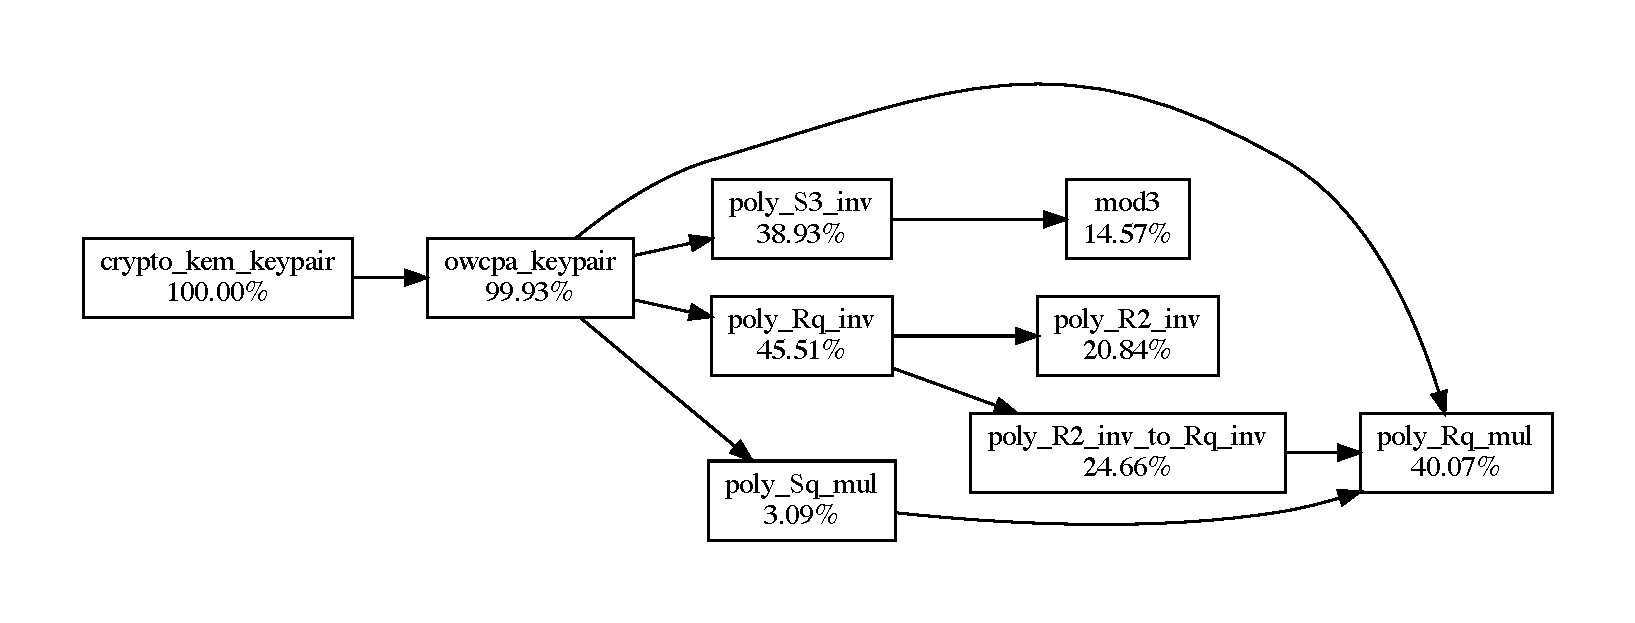
\includegraphics[scale=0.5]{chapters/results/hot-paths/ntru/crypto_kem_keypair.pdf}
    \caption{Relative instruction count of \gls{ntru}'s \textit{crypto\_kem\_keypair}}
    \label{figure:result:hot-paths:ntru:crypto_kem_keypair}
\end{figure}

Figure \ref{figure:result:hot-paths:ntru:crypto_kem_enc} describes the encapsulation API function. The key is generated using random bytes which are fed through 256-bit \gls{aes} in its Electronic Code Book (ECB) configuration to produce uniformly random bytes. Again, we see a significant percentage of the instructions spent in the polynomial library - in \textit{poly\_Rq\_mul}.

\begin{figure}[H]
    \centering
    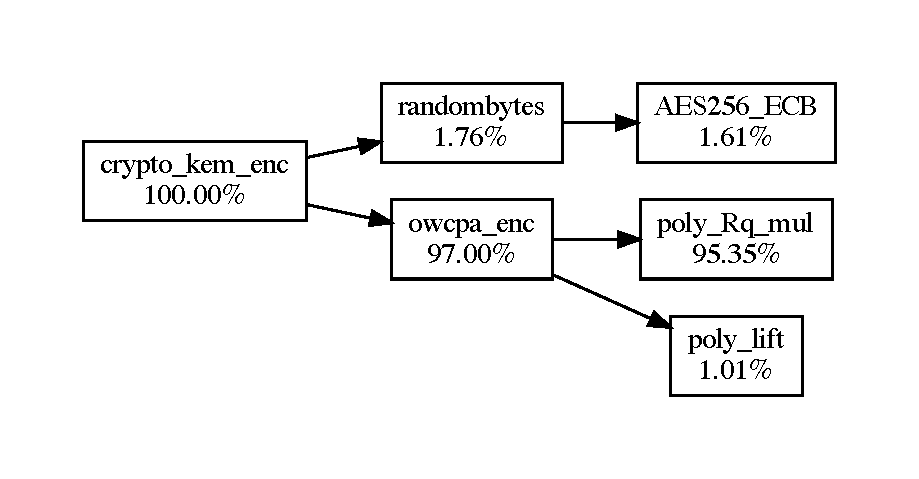
\includegraphics[scale=0.5]{chapters/results/hot-paths/ntru/crypto_kem_enc.pdf}
    \caption{Relative instruction count of \gls{ntru}'s \textit{crypto\_kem\_keypair}}
    \label{figure:result:hot-paths:ntru:crypto_kem_enc}
\end{figure}

The decryption function of \gls{ntru} is presented in figure \ref{figure:result:hot-paths:ntru:crypto_kem_dec}. Virtually all of the instructions spent decrypting (decapsulating) a key is spent in the \textit{poly\_Rq\_mul} function.

\begin{figure}[H]
    \centering
    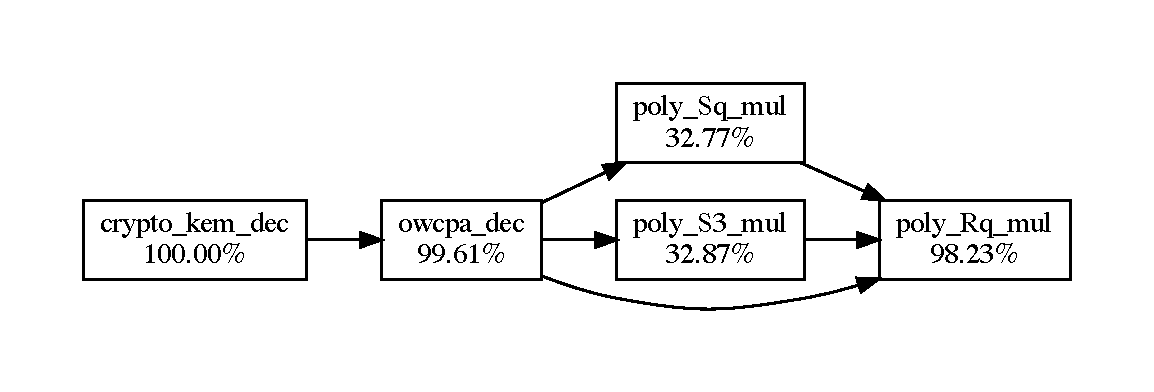
\includegraphics[scale=0.5]{chapters/results/hot-paths/ntru/crypto_kem_dec.pdf}
    \caption{Relative instruction count of \gls{ntru}'s \textit{crypto\_kem\_dec}}
    \label{figure:result:hot-paths:ntru:crypto_kem_dec}
\end{figure}

Looking at the code of \textit{poly\_Rq\_mul} as shown in figure \ref{figure:result:hot-paths:ntru:poly_Rq_mul}, it is evident that the vast majority of instructions are spent on multiplying and adding numbers in loops. The value of \textit{NTRU\_N} corresponds to the parameter set. For \gls{ntru} HRSS 701, the value is 701 and for \gls{ntru} HPS 4096821 the value is 821.

\begin{figure}[H]
    \centering
    \begin{lstlisting}[language=C]
void poly_Rq_mul(poly *r, const poly *a, const poly *b) {
  int k, i;

  for (k = 0; k < NTRU_N; k++) {
    r->coeffs[k] = 0;
    for (i = 1; i < NTRU_N - k; i++) // 10.21%
      r->coeffs[k] += a->coeffs[k + i] * b->coeffs[NTRU_N - i]; // 42.75%
    for (i = 0; i < k + 1; i++) // 8.20%
      r->coeffs[k] += a->coeffs[k - i] * b->coeffs[i]; // 38.79%
  }
}
    \end{lstlisting}
    \caption{Annotated source code of \gls{ntru}'s \textit{poly\_Rq\_mul}}
    \label{figure:result:hot-paths:ntru:poly_Rq_mul}
\end{figure}

To summarize, it is shown that factors such as the speed of \gls{aes} has little to do with the overall performance of the algorithm. Furthermore, it seems as if the polynomial library functions account for the vast majority of instructions spent on key-pair generation, encryption and decryption. The function \textit{poly\_Rq\_mul}, which multiplies two polynomials in $\mathbb{R}^q$, accounts for most of the calculations performed.

\subsubsection{Classic McEliece}
The \gls{mceliece} reference implementation consists of three API methods - \textit{crypto\_kem\_keypair}, \textit{crypto\_kem\_enc} and \textit{crypto\_kem\_dec} for key-pair generation, encryption (encapsulation) and decryption (decapsulation), respectively. These API functions may in turn call several internal functions. We will only present the hot-paths for the \gls{mceliece} 8192128 non-f variant because it can quite accurately represent the hot-paths for all \gls{mceliece} variants. In the appendix, all hot-paths can be found. 

In figure \ref{figure:result:hot-paths:classic-mceliece:crypto_kem_keypair}, we can see the \textit{crypto\_kem\_keypair} function and its only significant internal function, the \textit{pk\_gen} function that takes up 98.57\% of the execution time. In figure \ref{figure:result:hot-paths:classic-mceliece:pk_gen}, we can see the deeper look into the \textit{pk\_gen} function there we can see that all its internal functions and that they do not make up much of the instructions. Most of the instructions are inside of the \textit{pk\_gen} function itself.\todo{explain better}

\begin{figure}[H]
    \centering
    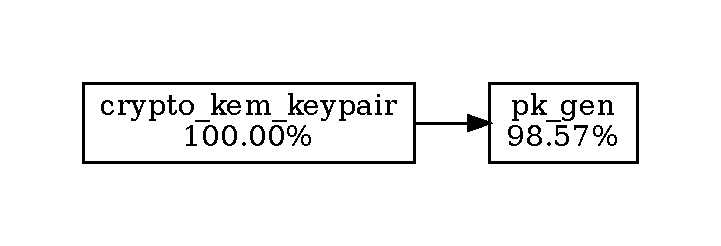
\includegraphics[scale=0.5]{chapters/results/hot-paths/classic-mceliece/8192128/crypto_kem_keypair.pdf}
    \caption{Relative instruction count of \gls{mceliece}'s \textit{crypto\_kem\_keypair}}
    \label{figure:result:hot-paths:classic-mceliece:crypto_kem_keypair}
\end{figure}

\begin{figure}[H]
    \centering
    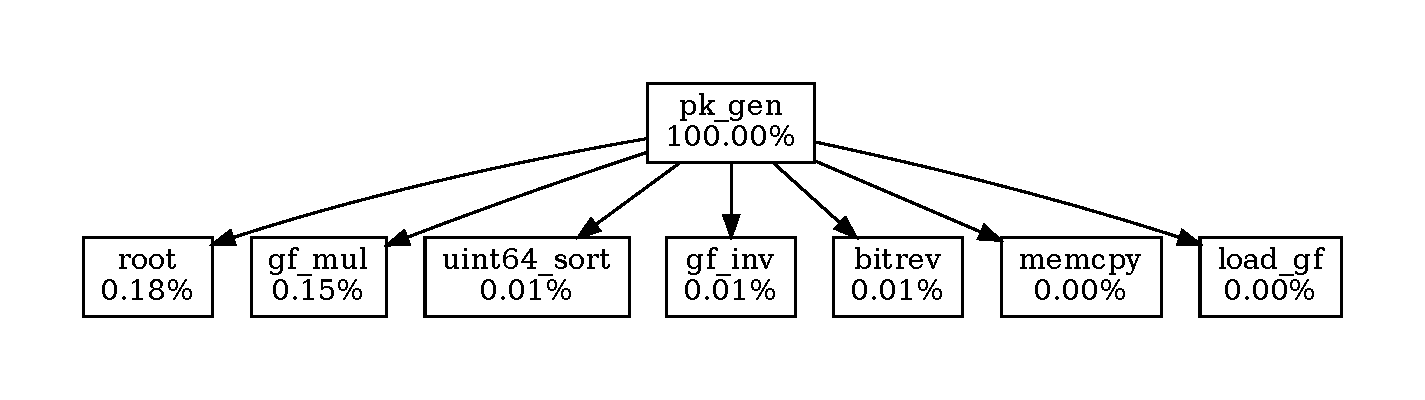
\includegraphics[scale=0.5]{chapters/results/hot-paths/classic-mceliece/8192128/pk_gen.pdf}
    \caption{Relative instruction count of \gls{mceliece}'s \textit{pk\_gen}}
    \label{figure:result:hot-paths:classic-mceliece:pk_gen}
\end{figure}

\begin{figure}[H]
    \centering
    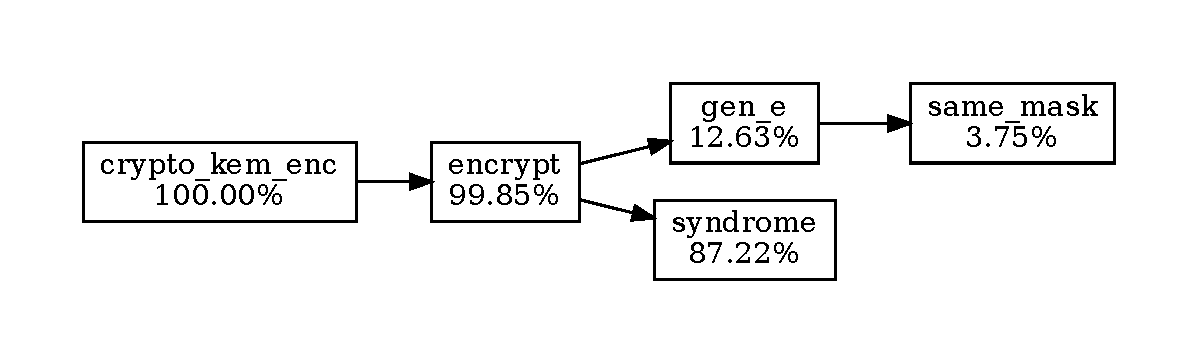
\includegraphics[scale=0.5]{chapters/results/hot-paths/classic-mceliece/8192128/crypto_kem_enc.pdf}
    \caption{Relative instruction count of \gls{mceliece}'s \textit{crypto\_kem\_keypair}}
    \label{figure:result:hot-paths:classic-mceliece:crypto_kem_enc}
\end{figure}

\begin{figure}[H]
    \centering
    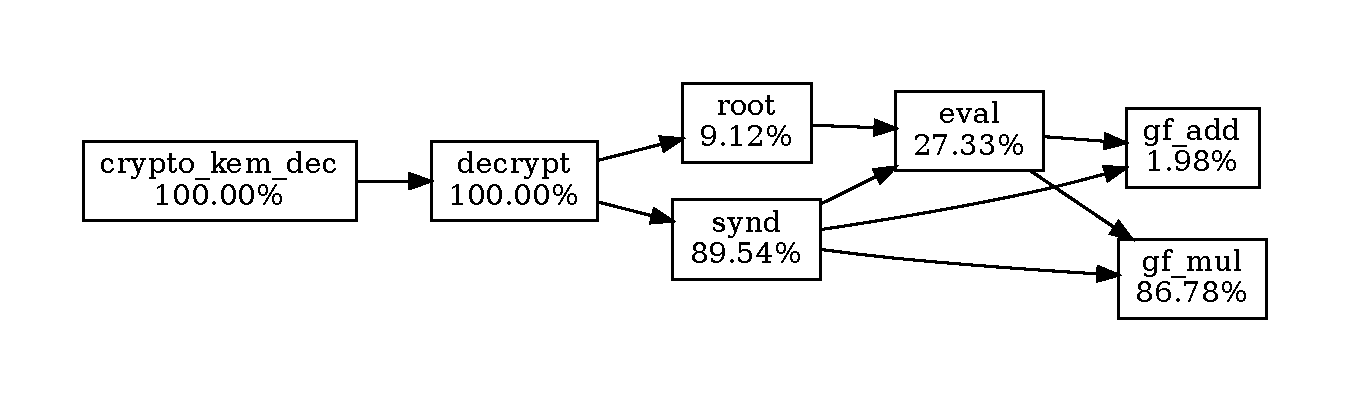
\includegraphics[scale=0.5]{chapters/results/hot-paths/classic-mceliece/8192128/crypto_kem_dec.pdf}
    \caption{Relative instruction count of \gls{mceliece}'s \textit{crypto\_kem\_dec}}
    \label{figure:result:hot-paths:classic-mceliece:crypto_kem_dec}
\end{figure}

\todo[inline]{Var tydliga med hot paths och tid. Exempelvis så lär diagrammet för pk\_gen visa 0\% för vissa funktioner så som root, men om vi ser till hot paths så lär vi se att de kallas flera miljoner gånger. Kanske ha en graf som visar antalet invocations?}

\todo[inline]{Ingen microbenchmark för eval, gf\_mul och gf\_add - de körs så många gånger att overheaden för profiling blev 1000x. McEliece kallar på många många tusen funktioner (hundra tusen, uppemot miljoner?) - det i sig bör ge mer overhead. }

\section{Post-Quantum Cryptography on z15}

\todo[inline]{
What specialized instructions and features applicable for post-quantum keyencapsulation mechanisms are available in z15 and how are they used in context?

Litteraturstudien.
}

\section{The Performance of Post-Quantum Key Exchange Mechanisms}

This section presents the results of the experiment as outlined in section \ref{section:method:experiment}. It further discusses the performance of \gls{post-quantum} \glspl{kem} and how they may differ on various architectures and hardware.

\subsection{Algorithm Performance}

In section \ref{section:method:experiment:phase1:implementation-configurations} it was written that the monitored functions for the micro benchmark would be based off of data found in the hot paths analysis. In the end, the functions presented in Table \ref{table:results:performance:micro-functions} were monitored during the micro benchmark. Note that although the randombytes function is available in both \gls{ntru} and \gls{mceliece}, it was found in section \ref{section:results:hot-paths} to not be significant enough to warrant further analysis.

\begin{table}[H]
    \centering
    \caption{Monitored Functions}
    \label{table:results:performance:micro-functions}
    \begin{tabularx}{\linewidth}{l X}
        \toprule
        \thead{Name} & \thead{Description} \\
        \midrule
        \multicolumn{3}{c}{\thead[l]{\gls{mceliece} and \gls{ntru}}} \\
        %\midrule
        crypto\_kem\_keypair & Generate a keypair \\
        crypto\_kem\_enc & Generate and encapsulate a key \\
        crypto\_kem\_dec & Decapsulate an encapsulated key \\
        \multicolumn{3}{c}{\thead[l]{\gls{mceliece}}} \\
        pk\_gen & \\
        gen\_e & \\
        syndrome & \\
        % syndrome\_asm & The same as syndrome, but implemented in assembly targeting AVX2\\
        root & \\
        synd & \\
        \multicolumn{3}{c}{\thead[l]{\gls{ntru}}} \\
        poly\_Rq\_mul & Multiply a polynomial with another in $\mathbb{R}_q$\\
        poly\_S3\_inv & Invert a polynomial in $\mathbb{S}_3$\\
        randombytes & Retrieve uniformly random bytes \\
        poly\_Rq\_inv & Invert a polynomial in $\mathbb{R}_2$\\
        poly\_R2\_inv & Invert a polynomial in $\mathbb{R}_2$\\
        poly\_R2\_inv\_to\_Rq\_inv & Lift an inverted polynomial from $\mathbb{R}_2$ to $\mathbb{R}_q$ \\
        poly\_Sq\_mul & Multiply a polynomial in $\mathbb{S}_q$ with another\\
        \bottomrule
    \end{tabularx}
\end{table}

\todo[inline]{
Does the performance of post-quantum key encapsulation mechanisms differ between architectures and if so, how?
What techniques may be used to increase the performance of post-quantum key encapsulation mechanisms?
}

\todo[inline]{
Talk about all the sequential data here - sequential, heap, micro, stack. Use all data, no matter the underlying system, to get an average of the state of the machines? If we only use relative measurements, that will be fine even though the i3 may lower the throughput?
}

\subsection{Hardware Performance}

\todo[inline]{
Does the performance of post-quantum key encapsulation mechanisms differ between architectures and if so, how?
What techniques may be used to increase the performance of post-quantum key encapsulation mechanisms?
}

\todo[inline]{
Talk about the parallel benchmark here, hardware throughput, hardware differences.
}

\subsection{Heap Usage}

As outlined in the method, section \ref{section:method:experiment:phase1:measurements}, we measured the heap usage of the algorithms by monitoring heap allocation and deallocation methods such as malloc using heaptrack. We found that the heap allocation did not change across environments nor between the analyzed optimizations except for some few . As for the implementations, this is rather unsurprising as changing how the allocations worked would alter the behavior of the code. As we found that the heap behavior of the algorithms were consistent throughout our test, we will for the rest of this section not refer to any specific environment or optimization used for the algorithms unless otherwise noted. When talking about allocation, we will refer to the peak allocation - that is, the maximum allocated bytes recorded during a function's lifetime. Our measurements did not capture the peak heap allocation during a benchmark as it would include memory allocations introduced by our tooling. The heap usage metrics do not reflect total memory usage as memory in the form of parameters passed to the algorithms or memory that's part of the stack is not included.

At one point, the \gls{ntru} implementations allocated $264$ bytes generating a keypair. These bytes were allocated by OpenSSL to initialize the library's envelope suite of functions. In context, this is done as the \gls{ntru} implementation uses OpenSSL's \gls{aes} ECB implementation to generate uniform pseduo-random bytes. The invocation of the \gls{aes} function itself resulted in $208$ bytes being allocated by the OpenSSL \gls{aes} ECB implementation. Beyond these bytes, the \gls{ntru} implementation did not require any additional heap allocation during its runtime.

Just like the \gls{ntru} implementations, the \gls{mceliece} implementations make use of OpenSSL to create uniform pseudo-random bytes. As such, the same $264$ bytes are allocated to initialize OpenSSL's envelope suite of functions, as well as the $208$ bytes to actually encrypt random data to produce a uniformly distributed series of bytes. No further allocations were found to be made.

The \gls{ecdhe} and \gls{dhe} implementations are based entirely on functions made available via the OpenSSL library. All of the implementations had an increase in the number of allocations made when compared to \gls{ntru} and \gls{mceliece}. The \gls{dhe} implementation when run in the IBM Community Cloud environment saw an allocation of $16960$ bytes during keypair generation made from a function to calculate the constant-time modulo exponentiation on an arbitrary large number. All other environments allocated $9024$ bytes for the same invocation. Furthermore, the keypair generation saw the allocation of a further $1024$ bytes in the IBM Community Cloud environment seemingly related to the same modulo operation.
The operation of dividing an integer was found to correlate to an additional $536$ bytes in the Cloud Provider 1 environment and $528$ bytes in all of the other environments. The environments saw an additional $1432$ bytes corresponding to the handling of arbitrary large numbers whilst generating a keypair. Fetching random data raised the allocation with $632$ bytes in all environments. There were further allocations made, all of which are summarized in Table \ref{table:results:memory:dhe-heap}. In the table, the peak heap usage of each function of the implementation has been summed up to produce a sum of peaks. This value does not correspond to the peak heap usage of the algorithm as a whole. The \gls{ecdhe} implementation behaved much like the \gls{dhe}, with the peaks differing between some environments. The implementation too worked with OpenSSL's arbitrary numbers and as such had several of the same allocations as the \gls{dhe} implementations. The peaks are presented in Table \ref{table:results:memory:ecdhe-heap}.

\begin{table}
    \centering
    \caption{Heap Allocation in Bytes for \gls{dhe}}
    \label{table:results:memory:dhe-heap}
    \begin{tabularx}{\linewidth}{X c c c}
        \toprule
        \thead{Environment} & \thead{OpenSSL Version} & \multicolumn{2}{c}{\thead{Sum of Peaks}}\\
        & & \thead{Keypair} & \thead{Exchange} \\
        \midrule
        IBM Community Cloud & 1.1.1g FIPS & 19772 & 19248 \\
        Cloud Provider 1 & 1.1.1 & 12076 & 12080 \\
        Cloud Provider 2 & 1.1.1f & 11852 & 11536\\
        Modern Workstation & 1.1.1f & 11852 & 11536 \\
        Modern Laptop & 1.1.1f & 11852 & 11536 \\
        Old Mid-Range Laptop & 1.1.1f & 11852 & 11536\\
        Old Low-Range Laptop & 1.1.1f & 11852 & 11536\\
        \bottomrule
    \end{tabularx}
\end{table}
\todo{correct values in table}

\begin{table}
    \centering
    \caption{Heap Allocation in Bytes for \gls{ecdhe}}
    \label{table:results:memory:ecdhe-heap}
    \begin{tabularx}{\linewidth}{X c c c c}
        \toprule
        \thead{Environment} & \thead{Curve} & \thead{OpenSSL Version} & \multicolumn{2}{c}{\thead{Sum of Peaks}}\\
        & & & \thead{Keypair} & \thead{Exchange} \\
        \midrule
        IBM Community Cloud & P-256 & 1.1.1g FIPS & 4920 & 1520 \\
        IBM Community Cloud & 25519 & 1.1.1g FIPS & 4524 & 1520 \\

        Cloud Provider 1 & P-256 & 1.1.1 & - & - \\
        Cloud Provider 1 & 25519 & 1.1.1 & - & - \\

        Cloud Provider 2 & P-256 & 1.1.1f & 2584 & 2136 \\
        Cloud Provider 2 & 25519 & 1.1.1f & 1192 & 2005\\

        Modern Workstation & P-256 & 1.1.1f & 2584 & 2136 \\
        Modern Workstation & 25519 & 1.1.1f & 1192 & 2005 \\
        
        Modern Laptop & P-256 & 1.1.1f & 2584 & 2136 \\
        Modern Laptop & 25519 & 1.1.1f & 1192 & 2005 \\
        
        Old Mid-Range Laptop & P-256 & 1.1.1f & 2584 & 2136\\
        Old Mid-Range Laptop & 25519 & 1.1.1f & 1192 & 2005\\
        
        Old Low-Range Laptop & P-256 & 1.1.1f & 2584 & 2136\\
        Old Low-Range Laptop & 25519 & 1.1.1f & 1192 & 2005\\
        \bottomrule
    \end{tabularx}
\end{table}
\todo{correct values in table}

\subsection{Stack Usage}

In terms of stack usage, the results vary between the implementations, compilers and features. For instance, the polynomial math function poly\_Rq\_mul in \gls{ntru}, which was identified as constituting most of the time spent in the algorithm, varies between taking up $70499$ and $188$ bytes. In all environments, the HPS 4096821 AVX2 variant takes up $70499$ bytes. This does not change between compilers or optimization flags, which could be due to the fact that the implementation is written in assembly - leaving little room for the compiler to alter the behavior. The same goes for the HRSS 701 variant of \gls{ntru} - the size is consistently $55317$ across environments and optimization flags. The lowest sizes are found when the reference implementation is compiled with optimization. The sizes are presented in Table \ref{table:results:memory:ntru-stack}. Although the optimization flags used were not chosen for improving the size of the binary, the size of the function has been lowered in all cases. Although the same version of GCC was used for several environments, the results differed between $188$ and $192$ bytes. Clang continually produced larger regions than GCC. Furthermore, more recent versions of the compilers seem to have produced smaller sizes.

\begin{table}
    \centering
    \caption{Stack Size of poly\_Rq\_mul in Bytes for the Optimized Reference Implementation}
    \label{table:results:memory:ntru-stack}
    \begin{tabularx}{\linewidth}{X c c c c}
        \toprule
        \thead{Environment} & \thead{Compiler} & \thead{Compiler Version} & \thead{Optimized Size} & \thead{Reference Size}\\
        \midrule
        Cloud Provider 1 & clang & 6.0.0 & 702 & N/A \\
        IBM Community Cloud & clang & 10.0.1 & 522 & N/A \\
        Cloud Provider 2 & clang & 10.0.0 & 380 & N/A \\
        Modern Laptop & clang & 10.0.0 & 380 & N/A \\
        Modern Workstation & clang & 10.0.0 & 380 & N/A \\
        Cloud Provider 2 & clang & 10.0.0 & 380 & N/A \\
        Modern Laptop & clang & 10.0.0 & 380 & N/A \\
        Old Low-Range Laptop & clang & 10.0.0 & 300 & N/A \\
        Old Mid-Range Laptop & clang & 10.0.0 & 300 & N/A \\
    
        IBM Community Cloud & gcc & 8.3.1 & 242 & 382 \\
        Old Low-Range Laptop & gcc & 9.3.0 & 196 & 255 \\
        Old Mid-Range Laptop & gcc & 9.3.0 & 196 & 255 \\
        Cloud Provider 1 & gcc & 7.5.0 & 192 & 253\\
        Cloud Provider 2 & gcc & 9.3.0 & 188 & 255\\
        Modern Laptop & gcc & 9.3.0 & 188 & 255\\
        Modern Workstation & gcc & 9.3.0 & 188 & 255\\
        \bottomrule
    \end{tabularx}
\end{table}

The same correlation between optimization flags and compiler versions could not be found in the case of \gls{mceliece} and pk\_gen. In that case, the largest recorded size was found in IBM Community Cloud's optimized reference implementation with $22858$ bytes. The optimized AVX2 implementation of the Modern Workstation and Modern Laptop came second with $22123$ bytes. Lastly, the smallest size recorded was found in the optimized reference implementation of Old Mid-Range Laptop and Old Low-Range Laptop at $2026$ bytes.

As for other functions of the \glspl{kem}, the data is too massive to comprehensively refer to here. There are, however, tables in the appendix for average sizes as compared to the reference implementation compiled with GCC. In Table \ref{table:result:ntru-average-stack-increase-cloud}, for example, one may see that Clang seems to produce smaller binaries. Furthermore, the optimized AVX2 build results in the largest binaries - with symbols taking 8-10 times the size of the reference implementation.

\todo[inline]{Discuss stack usage of ECDHE, DHE?}

\subsection{Parameter Sizes}

The measurements presented up until this point have been related to either the runtime behavior of the algorithms, or the static requirements they place on the environment. These measurements have not included the parameters fed to the algorithms - which could affect real-world applications. The remaining part of this section will present data gathered from the various implementations.

The \glspl{kem} tested conform to the same API. Their signatures are presented in figure \ref{figure:result:memory:kem-api}. The function crypto\_kem\_keypair, which generates a keypair takes in a public key and a secret key. The encapsulation function, crypto\_kem\_enc, takes in a ciphertext buffer, a key buffer and the public key of a peer. Lastly, the decapsulation function, crypto\_kem\_dec takes in a key buffer, the ciphertext as received from a peer and the secret key. The sizes of these parameters differ between algorithms and implementations - but is not changed depending on the environment or optimizations. Table \ref{table:results:memory:kem-parameter-sizes} shows the sizes of the parameters in bytes. The sizes do not differ between the "f" variants of \gls{mceliece}. Therefore only two variants of \gls{mceliece} are presented.

\begin{figure}
    \centering
    \begin{lstlisting}[language=C]
int crypto_kem_keypair(unsigned char *public_key, unsigned char *private_key);
int crypto_kem_enc(unsigned char *ciphertext, unsigned char *key, const unsigned char *public_key);
int crypto_kem_dec(unsigned char *key, const unsigned char *ciphertext, const unsigned char *private_key);
    \end{lstlisting}
    \caption{The API of the \gls{kem} Implementations}
    \label{figure:result:memory:kem-api}
\end{figure}

\begin{table}
    \centering
    \caption{Parameter Sizes in Bytes of the \glspl{kem} Under Test}
    \label{table:results:memory:kem-parameter-sizes}
    \begin{tabularx}{\linewidth}{X c c c c c}
        \toprule
        \thead{Algorithm} & \thead{Parameters} & \thead{public\_key} & \thead{private\_key} & \thead{ciphertext} & \thead{key}\\
        \midrule
        \gls{mceliece} & 8192128(f) & 1357824 & 14120 & 240 & 32 \\
        \gls{mceliece} & 6960119(f) & 1047319 & 13948 & 226 & 32 \\
        \gls{ntru} & HRSS 701 & 1138 & 1450 & 1138 & 32 \\
        \gls{ntru} & HPS 4096821 & 1230 & 1590 & 1230 & 32 \\
        \bottomrule
    \end{tabularx}
\end{table}

The APIs are similar, but not the same for the \gls{kex} implementations. That is due to \gls{dh} requiring the so called Diffie-Hellman Parameters $p$ and $g$. The APIs are shown in figure \ref{figure:results:memory:kex-api}. As with the \gls{kem} implementations, the \gls{kex} implementations use two buffers for a public and a private key when generating a keypair. The \gls{dh} implementation also requires the previously mentioned domain parameters $p$ and $g$ - both buffers of bytes containing the respective parameter. The crypto\_dh\_enc functions further use a key buffer. There is no analogous ciphertext as the \glspl{kex} are fundamentally different from the \glspl{kem} as covered in \ref{section:background:diffie-hellman}. The sizes of the parameters are presented in Table \ref{table:results:memory:kex-parameter-sizes}.

\begin{figure}
    \centering
    \begin{lstlisting}[language=C]
// Diffie-Hellman
int crypto_dh_keypair(unsigned char *public_key, unsigned char *private_key, unsigned char *p, unsigned char *g);

// Diffie-Hellman
int crypto_dh_enc(unsigned char *key, const unsigned char *private_key, const unsigned char *public_key, unsigned char *p, unsigned char *g);

// Elliptic-Curve Diffie-Hellman
int crypto_dh_keypair(unsigned char *public_key, unsigned char *private_key);

// Elliptic-Curve Diffie-Hellman
int crypto_dh_enc(unsigned char *key, const unsigned char *private_key, const unsigned char *public_key);
    \end{lstlisting}
    \caption{The API of the \gls{kex} Implementations}
    \label{figure:results:memory:kex-api}
\end{figure}

\begin{table}
    \centering
    \caption{Parameter Sizes in Bytes of the \glspl{kex} Under Test}
    \label{table:results:memory:kex-parameter-sizes}
    \begin{tabularx}{\linewidth}{X c c c c c c}
        \toprule
        \thead{Algorithm} & \thead{Parameters} & \thead{public\_key} & \thead{private\_key} & \thead{$p$} & \thead{$g$} & \thead{key}\\
        \midrule
        \gls{dh} & 2048    &255 & 255 & 256  & 1 & 32 \\
        \gls{ecdh} & P-256 & 65 & 32 & - & - & 32 \\
        \gls{ecdh} & 25519 & 32 & 32 & - & - & 32 \\
        \bottomrule
    \end{tabularx}
\end{table}

\subsection{Sequential Performance}

The performance of the algorithms were analyzed by performing a thousand sequential runs in series, for each algorithm under test. The complete method is outlined in section \ref{section:method:experiment:phase1}.

As covered in section \ref{section:background:mceliece}, \gls{mceliece} supports two forms of keypair-generation algorithms - a non-systematic form and a semi-systematic form. The authors of the \gls{nist} submission state that these two forms may have different performance characteristics \cite{mceliece2020}. In Table \ref{table:results:sequential-mceliece-6960119-keypair-modern-workstation}, these two forms can be seen with every set of performance improvements tested in the experiment. As can bee seen in the table, the reference implementation in its non-systematic form is remarkably inconsistent, with a standard deviation of $20580.20$ as compared to the $6.91$ of the semi-systematic form. The change in performance characteristics is also visible in the mean, with the semi-systematic form taking about $30\%$ of the time on average as compared to the non-systematic form. In both cases, the \gls{avx2} implementation has the second largest standard deviation with $302.58$ and $6.91$ for the non-systematic form and the semi-systematic form, respectively. Despite being a \gls{simd} implementation, \gls{avx2} performs worse than the optimized reference implementation in both forms of the algorithm. The optimized \gls{avx2}, however, outperforms the optimized reference implementation with a 4-6 times the performance. The same results were found to generalize for several environments, as shown in Table \ref{table:results:sequential:mceliece-6960119-keypair} and \ref{table:results:sequential:mceliece-6960119f-keypair}.

\begin{table}
    \centering
    \caption{Duration of \gls{mceliece} 6960119 Keypair Generation On Modern Workstation}
    \label{table:results:sequential-mceliece-6960119-keypair-modern-workstation}
    \begin{tabularx}{\linewidth}{l X c c c c}
        \toprule
        \thead{Compiler} & \thead{Flags} & \thead{Mean} & \thead{Standard\\Deviation} & \multicolumn{2}{c}{\thead{95\% CI}}\\
        & & & & \thead{Lower} & \thead{Upper} \\
        \midrule
        \thead{non-systematic form}\\
                         gcc &                  ref &             21885.78 &             20580.20 &             17376.37 &             26395.19\\
                         gcc &                 avx2 &               562.39 &               302.58 &               549.13 &               575.66\\
                       clang &        ref-optimized &               696.65 &               571.35 &               671.60 &               721.70\\
                         gcc &        ref-optimized &               421.15 &               317.77 &               407.22 &               435.09\\
                         gcc &       avx2-optimized &                72.26 &                38.78 &                70.56 &                73.96\\
                       clang &       avx2-optimized &                70.28 &                38.12 &                68.61 &                71.95\\
    
    \midrule
      \thead{semi-systematic form}\\
                        gcc &                  ref &              6476.15 &                 6.91 &              6475.33 &              6476.97\\
                         gcc &                 avx2 &               315.24 &                 0.96 &               315.19 &               315.28\\
                       clang &        ref-optimized &               230.14 &                 0.74 &               230.11 &               230.18\\
                         gcc &        ref-optimized &               159.12 &                 0.61 &               159.09 &               159.15\\
                         gcc &       avx2-optimized &                40.45 &                 0.84 &                40.42 &                40.49\\
                       clang &       avx2-optimized &                39.93 &                 1.50 &                39.86 &                39.99\\
        \bottomrule
    \end{tabularx}
\end{table}

In all environments but one, we found a consistent performance throughout all sequential runs, non-deterministic behavior and outliers aside. The Cloud Provider 2 environment provided inconsistent results throughout the sequential performance benchmarks - across various algorithms and runs. As seen in figure \ref{figure:results:sequential:mceliece-decrpyt-cloud-provider-2}, there are several occasions where the performance shift over time. In the figure, the speedup relative to the reference GCC implementation is used as opposed to the absolute duration of each iteration. Depending on how deterministic the behavior of the algorithms are, as well as how stable the environment is, one could have expected more or less the same performance throughout the test. As the Cloud Provider 2 environment uses two virtual CPU cores, it is not entirely unexpected to find such inconsistent results. No evidence was found regarding the same behavior in the environments tested with dedicated hardware.

\begin{figure}
    \centering
    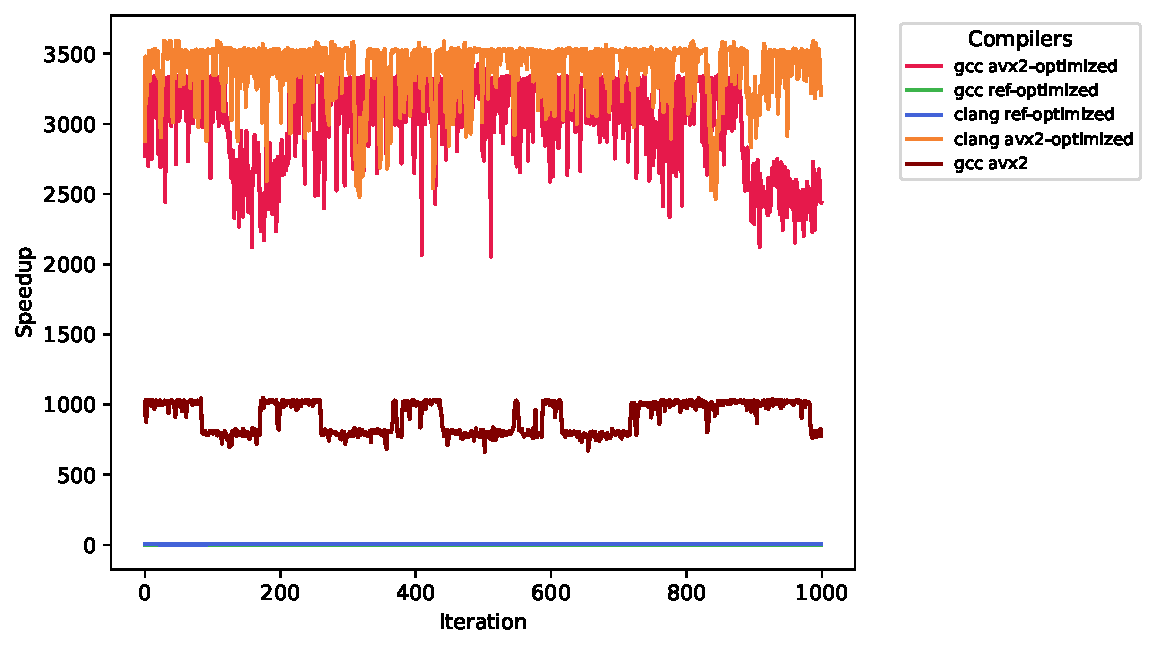
\includegraphics[scale=0.75]{chapters/results/sequential/mceliece_6960119_decrypt_Cloud Provider 2.pdf}
    \caption{The Speedup of \gls{mceliece} 6960119 Using Various Performance Changes Over Time}
    \label{figure:results:sequential:mceliece-decrpyt-cloud-provider-2}
\end{figure}

% sequential runs table på någon eller några algoritmer? Jämför speedup - bör vara samma då den är procentuell. Man kan se om en miljö må bra av en viss ändring i jämförelse med andra.
% TODO: få in data från keypair, encrypt och decrypt i samma graf!
% Carl fixar
\begin{table}
    \centering
    \caption{Sequential Runs for ntru hrss701 (encrypt)}
    \begin{tabularx}{\linewidth}{X c c c c c}
        \toprule
        \thead{Environment} & \thead{Compiler} & \thead{Flags} & \thead{Average Duration} & \thead{Speedup}\\
        \midrule
          Modern Workstation &                  gcc &                  ref &  0.91ms &                  0.0\\
          Modern Workstation &                  gcc &        ref-optimized &  0.23ms &                  2.9\\
          Modern Workstation &                clang &        ref-optimized &  0.21ms &                  3.4\\
          Modern Workstation &                  gcc &                 avx2 &  0.03ms &                 30.8\\
          Modern Workstation &                  gcc &       avx2-optimized &  0.02ms &                 49.7\\
          Modern Workstation &                clang &       avx2-optimized &  0.02ms &                 54.3\\
               Modern Laptop &                  gcc &                  ref &  1.15ms &                  0.0\\
               Modern Laptop &                clang &        ref-optimized &  0.26ms &                  3.4\\
               Modern Laptop &                  gcc &        ref-optimized &  0.28ms &                  3.1\\
               Modern Laptop &                  gcc &                 avx2 &  0.05ms &                 21.5\\
               Modern Laptop &                  gcc &       avx2-optimized &  0.03ms &                 42.5\\
               Modern Laptop &                clang &       avx2-optimized &  0.02ms &                 46.1\\
        Old Mid-Range Laptop &                  gcc &                  ref &  1.58ms &                  0.0\\
        Old Mid-Range Laptop &                clang &        ref-optimized &  0.48ms &                  2.3\\
        Old Mid-Range Laptop &                  gcc &        ref-optimized &  0.42ms &                  2.8\\
        Old Low-Range Laptop &                  gcc &                  ref &  1.95ms &                  0.0\\
        Old Low-Range Laptop &                clang &        ref-optimized &  0.60ms &                  2.3\\
        Old Low-Range Laptop &                  gcc &        ref-optimized &  0.50ms &                  2.9\\
            Cloud Provider 1 &                  gcc &                  ref &  1.35ms &                  0.0\\
            Cloud Provider 1 &                  gcc &        ref-optimized &  0.39ms &                  2.4\\
            Cloud Provider 1 &                clang &        ref-optimized &  0.29ms &                  3.7\\
            Cloud Provider 1 &                  gcc &                 avx2 &  0.06ms &                 23.3\\
            Cloud Provider 1 &                clang &       avx2-optimized &  0.03ms &                 43.1\\
            Cloud Provider 1 &                  gcc &       avx2-optimized &  0.03ms &                 49.8\\
            Cloud Provider 2 &                  gcc &                  ref &  1.59ms &                  0.0\\
            Cloud Provider 2 &                  gcc &        ref-optimized &  0.40ms &                  2.9\\
            Cloud Provider 2 &                clang &        ref-optimized &  0.37ms &                  3.3\\
            Cloud Provider 2 &                  gcc &       avx2-optimized &  0.06ms &                 26.9\\
            Cloud Provider 2 &                  gcc &                 avx2 &  0.05ms &                 30.5\\
            Cloud Provider 2 &                clang &       avx2-optimized &  0.04ms &                 42.3\\
         IBM Community Cloud &                  gcc &                  ref &  2.11ms &                  0.0\\
         IBM Community Cloud &                  gcc &        ref-optimized &  0.49ms &                  3.3\\
         IBM Community Cloud &                clang &        ref-optimized &  0.39ms &                  4.4 \\
        \bottomrule
    \end{tabularx}
\end{table}

% TODO: använd samma tabell för alla algoritmer i appendix och referera till dem:
% sequential runs table  eller graf för att styrka upp och sammanfatta varför vi valde en algoritm / optimering för att köra parallelt.

\subsection{Throughput Performance}

% DH planar alltid ut exakt vid (fysisk|virtuell) core count
\begin{figure}
    \centering
    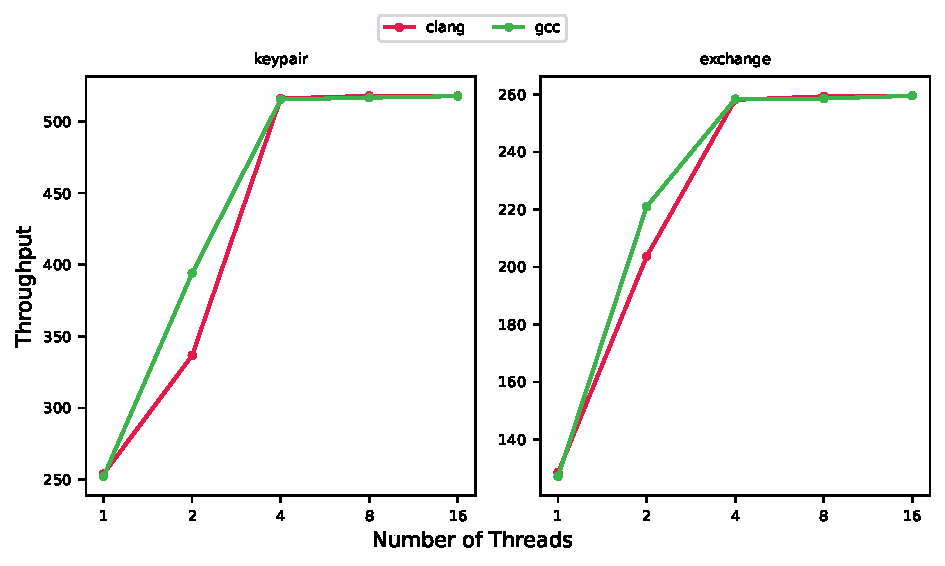
\includegraphics{chapters/results/throughput/Old Mid-Range Laptop_dh.pdf}
    \caption{Caption}
    \label{figure:results:throughput:dh-old-mid-range-laptop}
\end{figure}

% **IBM rejäl dipp 25% vid 2x smt för gcc 25519. IBM mycket snabbare än alla andra vid två kärnor - 339x för 25519 båda kompilatorerna. WTF?! 114-142x på ecdh exchange. p-256 dock snabbast. p-256 även den bra i keypair! Fortfarande riktigt bra i exchange. Dippen är konsekvent över två körningar! Så gott som exakt samma resultat för dippen på två helt olika körningar. Två trådar presterar i båda fallen hälften så bra som övriga två. Datan validerad. ** Motiverar i discussion och conclusion. Viktigt!
\begin{figure}
    \centering
    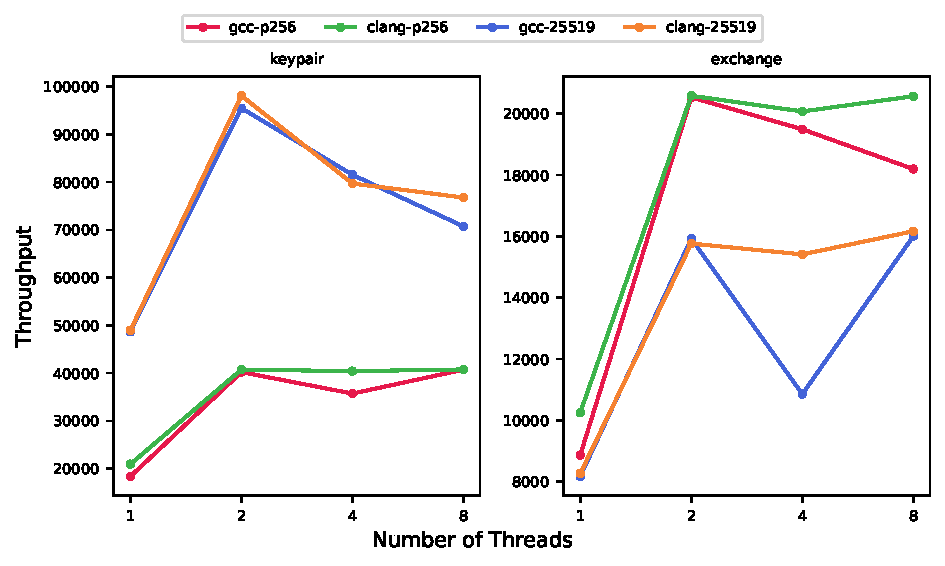
\includegraphics{chapters/results/throughput/IBM Community Cloud_ecdh.pdf}
    \caption{Caption}
    \label{figure:results:throughput:ecdh-ibm-community-cloud}
\end{figure}

% **IBM decrypt oerhört mycket långsammare än encrypt, något vi inte sett på andra environments. Andra har typ 70% performance, IBM typ >1%.** Grafer?
\begin{figure}
    \centering
    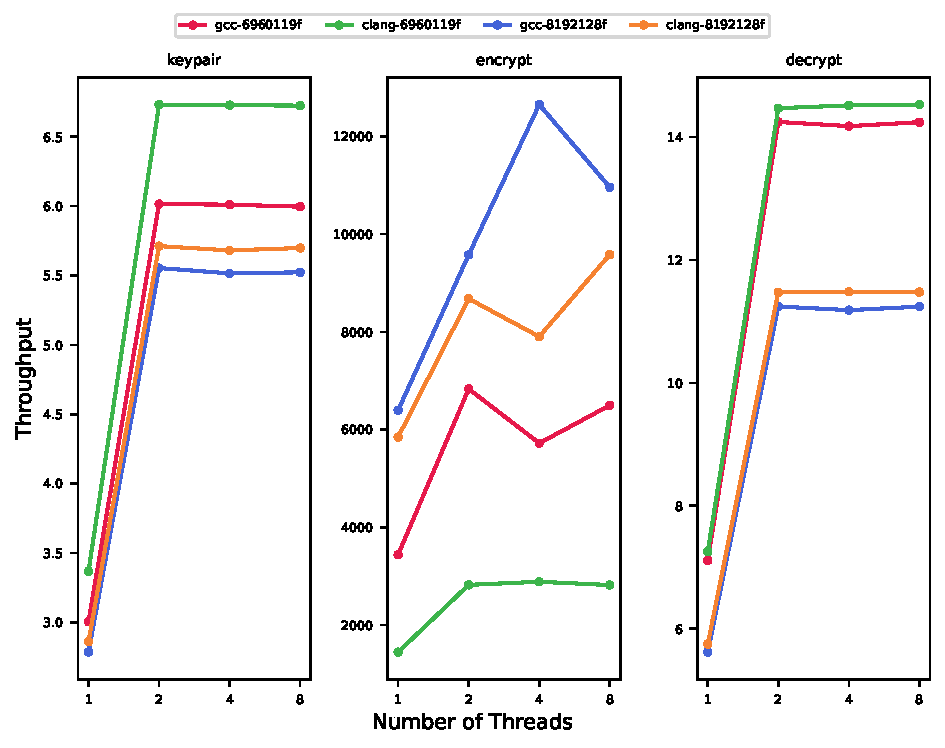
\includegraphics{chapters/results/throughput/IBM Community Cloud_mceliece.pdf}
    \caption{Caption}
    \label{figure:results:throughput:ibm-community-cloud}
\end{figure}

% Samma sak - antagligen avsaknad av AVX2 som gör det
\begin{figure}
    \centering
    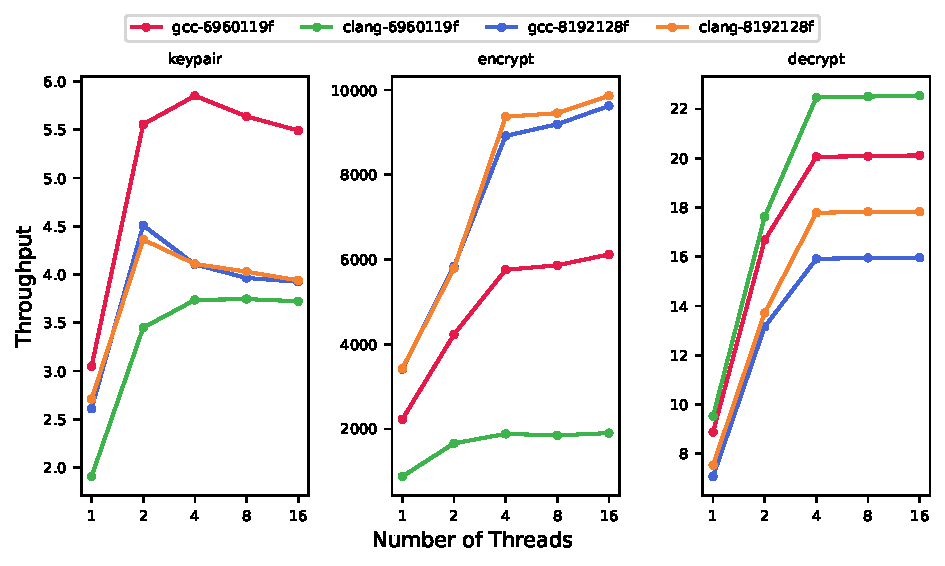
\includegraphics{chapters/results/throughput/Old Mid-Range Laptop_mceliece.pdf}
    \caption{Caption}
    \label{figure:results:throughput:mceliece-old-mid-range-laptop}
\end{figure}

% Jämför värdena med dessa - som har AVX2?
\begin{figure}
    \centering
    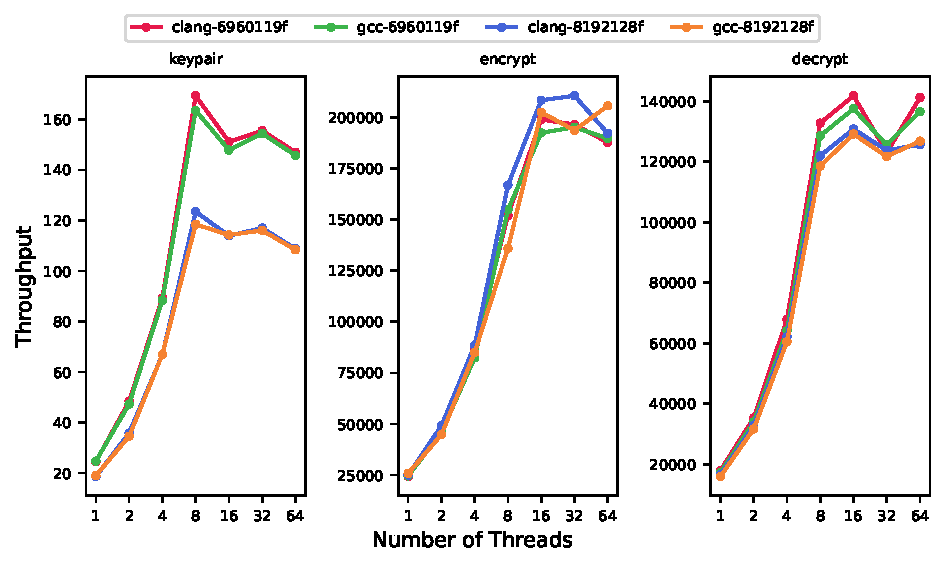
\includegraphics{chapters/results/throughput/Modern Workstation_mceliece.pdf}
    \caption{Caption}
    \label{figure:results:throughput:mceliece-modern-workstation}
\end{figure}

% **Modern Laptop, Modern Workstation - liknande, skalar bra per tråd, HRSS mycket snabbare än HPS4096821. Väldigt lika i decrypt, men inte encrypt eller keypair.** Grafer?
\begin{figure}
    \centering
    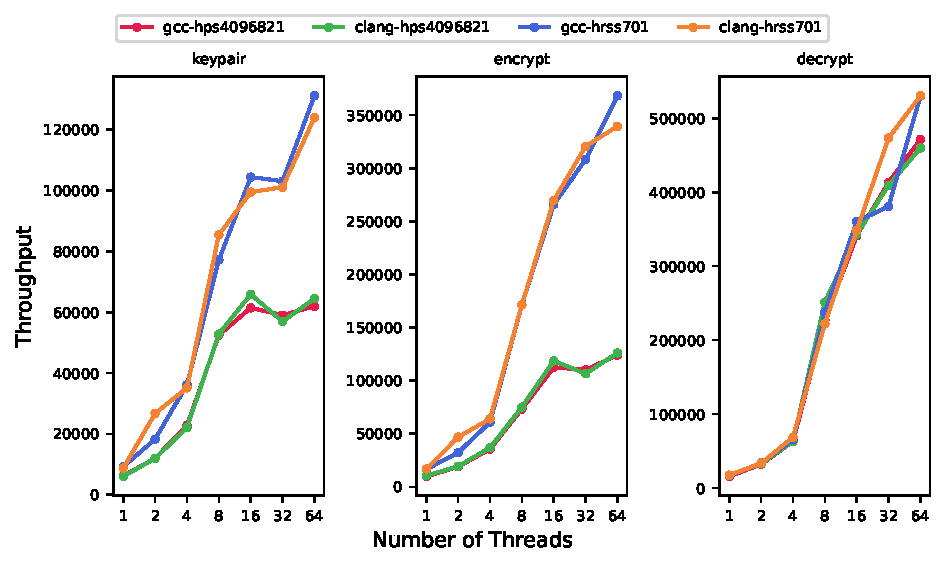
\includegraphics{chapters/results/throughput/Modern Workstation_ntru.pdf}
    \caption{Caption}
    \label{figure:results:throughput:ntru-modern-workstation}
\end{figure}

% NTRU hrss701 decrypt tabell? Bra skalning för modern *
    \begin{table}[H]
        \centering
        \small
        \caption{Parallel Throughput Runs for ntru hrss701 (decrypt)}
        \label{table:results:throughput:ntru-hrss701-decrypt}
        \begin{tabularx}{\linewidth}{X c c c c c c c c}
            \toprule
            \thead{Environment} & \thead{Compiler} & \multicolumn{7}{c}{\thead{Threads}}\\
            & & 1 & 2 & 4 & 8 & 16 & 32 & 64 \\
            \midrule
\multirowcell{4}{Cloud\\ Provider\\ 1 \footref{avx2-optimized}} & 
\multirow{2}{*}{gcc} & 47064 & 94918 & 94690 & 101730 & 103827\\
 & & 1.0 & 2.02 & 2.01 & 2.16 & 2.21\\
\cmidrule[0.05em](){3-9} & 
\multirow{2}{*}{clang} & 39753 & 71637 & 82847 & 85968 & 85693\\
 & & 0.84 & 1.52 & 1.76 & 1.83 & 1.82\\
            \midrule
\multirowcell{4}{Cloud\\ Provider\\ 2 \footref{avx2-optimized}} & 
\multirow{2}{*}{gcc} & 33224 & 68890 & 74596 & 64194\\
 & & 1.0 & 2.07 & 2.25 & 1.93\\
\cmidrule[0.05em](){3-9} & 
\multirow{2}{*}{clang} & 39840 & 69277 & 62418 & 75534\\
 & & 1.20 & 2.09 & 1.88 & 2.27\\
            \midrule
\multirowcell{4}{IBM\\ Community\\ Cloud \footref{ref-optimized}} & 
\multirow{2}{*}{gcc} & 705 & 1056 & 1373 & 1401\\
 & & 1.0 & 1.50 & 1.95 & 1.99\\
\cmidrule[0.05em](){3-9} & 
\multirow{2}{*}{clang} & 881 & 1772 & 1735 & 1745\\
 & & 1.25 & 2.51 & 2.46 & 2.47\\
            \midrule
\multirowcell{4}{Modern\\ Laptop \footref{avx2-optimized}} & 
\multirow{2}{*}{gcc} & 14694 & 26965 & 94495 & 147789 & 172734 & 176251\\
 & & 1.0 & 1.84 & 6.43 & 10.06 & 11.75 & 11.99\\
\cmidrule[0.05em](){3-9} & 
\multirow{2}{*}{clang} & 13041 & 32001 & 87645 & 104470 & 148045 & 166157\\
 & & 0.89 & 2.18 & 5.96 & 7.11 & 10.07 & 11.31\\
            \midrule
\multirowcell{4}{Modern\\ Workstation \footref{avx2-optimized}} & 
\multirow{2}{*}{gcc} & 16668 & 33956 & 65296 & 237728 & 360264 & 380808 & 530159\\
 & & 1.0 & 2.04 & 3.92 & 14.26 & 21.61 & 22.85 & 31.81\\
\cmidrule[0.05em](){3-9} & 
\multirow{2}{*}{clang} & 17454 & 33662 & 68787 & 222164 & 348442 & 473293 & 530368\\
 & & 1.05 & 2.02 & 4.13 & 13.33 & 20.90 & 28.39 & 31.82\\
            \midrule
\multirowcell{4}{Old\\ Low-Range\\ Laptop \footref{ref-optimized}} & 
\multirow{2}{*}{gcc} & 688 & 1286 & 1492 & 1476 & 1489\\
 & & 1.0 & 1.87 & 2.17 & 2.14 & 2.16\\
\cmidrule[0.05em](){3-9} & 
\multirow{2}{*}{clang} & 583 & 1102 & 1222 & 1219 & 1218\\
 & & 0.85 & 1.60 & 1.77 & 1.77 & 1.77\\
            \midrule
\multirowcell{4}{Old\\ Mid-Range\\ Laptop \footref{ref-optimized}} & 
\multirow{2}{*}{gcc} & 873 & 941 & 1762 & 1748 & 1781\\
 & & 1.0 & 1.08 & 2.02 & 2.00 & 2.04\\
\cmidrule[0.05em](){3-9} & 
\multirow{2}{*}{clang} & 767 & 1299 & 1512 & 1515 & 1518\\
 & & 0.88 & 1.49 & 1.73 & 1.73 & 1.74 \\
            \bottomrule
        \end{tabularx}
    \end{table}
    \addtocounter{footnote}{1}
    \footnotetext{\label{ref-optimized}ref-optimized}
    \addtocounter{footnote}{1}
    \footnotetext{\label{avx2-optimized}avx2-optimized}
    

\subsection{Throughput Performance}

As outlined in section \ref{section:method:experiment:phase2}, the throughput of the algorithms in each environment under test was evaluated for a series of parallelism configurations. The initial plan was to use the best-performing algorithm for each environment, as identified by the sequential benchmarks. Early results, however, were not conclusive and we therefore ended up running the parallel benchmarks on both GCC and Clang builds of the best-performing variant. The throughput of the algorithms differed depending on the environment and compiler used. The lowest throughput was found in Clang builds in the Old Low-Range Laptop, for which runs are presented in figure \ref{figure:results:throughput:mceliece:old-low-range-laptop} and figure \ref{figure:results:throughput:ntru:old-low-range-laptop}. As can be seen in figure \ref{figure:results:throughput:mceliece:old-low-range-laptop}, Clang yielded down to one fifth of the encryption throughput of the comparable GCC build, but also resulted in a roughly 5\% speedup over the comparable GCC implementation. In the \gls{ntru} tests, as presented in figure \ref{figure:results:throughput:ntru:old-low-range-laptop}, Clang produced a 50\% lower keypair throughput, 20\% lower encryption and decryption throughput than comparable versions compiled with GCC. A similar difference in throughput was also found in the Old Mid-Range Laptop and the IBM Community Cloud environments. All of these environments ran the optimized reference implementation due to lack of \gls{avx2} support.

\begin{figure}
    \centering
    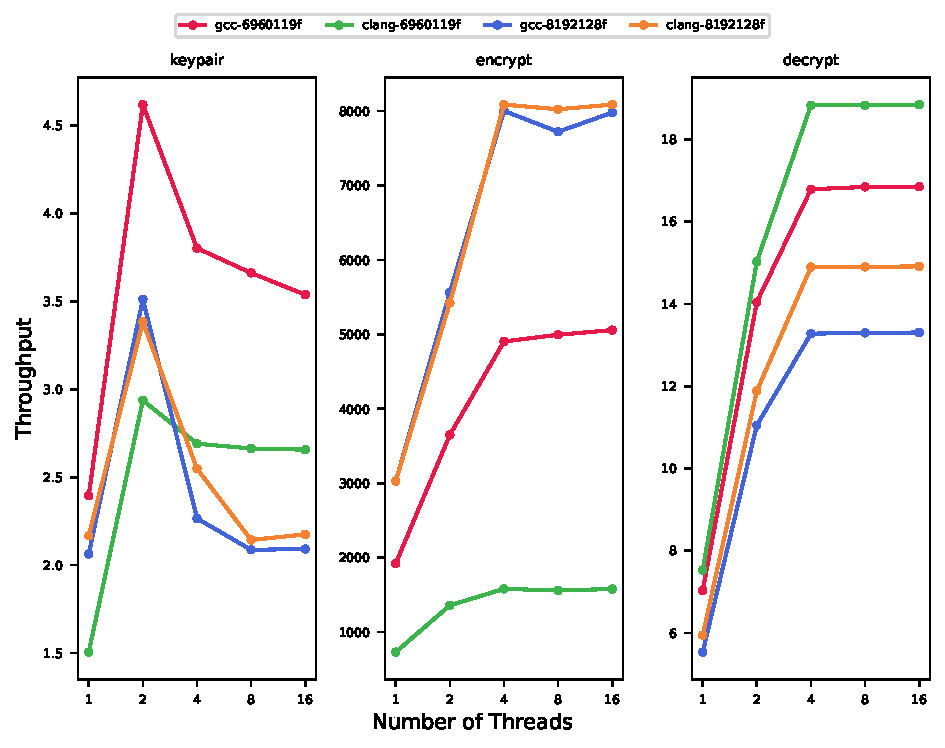
\includegraphics[scale=0.75]{chapters/results/throughput/Old Low-Range Laptop_mceliece.pdf}
    \caption{Throughput of \gls{mceliece} on Old Low-Range Laptop}
    \label{figure:results:throughput:mceliece:old-low-range-laptop}
\end{figure}

In the other end of the spectrum, we found the highest throughput in the Modern Workstation. Unlike the Old Low-Range Laptop, the Old Mid-Range Laptop and the IBM Community Cloud environments, the Modern Workstation ran the optimized \gls{avx2} binaries. Unlike the data presented in previous figures, figure \ref{figure:results:throughput:mceliece:modern-workstation} and figure \ref{figure:results:throughput:ntru:modern-workstation} show more consistent measurements. There seems to be little to no difference in speed between the GCC and Clang builds. In all stages of the algorithms, there seems to be a regression in throughput when using either 16 or 32 threads. The HRSS 701 variant of \gls{ntru} seems to have near linear scaling for the number of threads used in our tests. The \gls{mceliece} variants, however, seem to reach peak performance when using between 8 to 16 threads, with performance staying roughly the same for higher thread counts. The same scaling was also seen in the Modern Laptop environment.

\begin{figure}
    \centering
    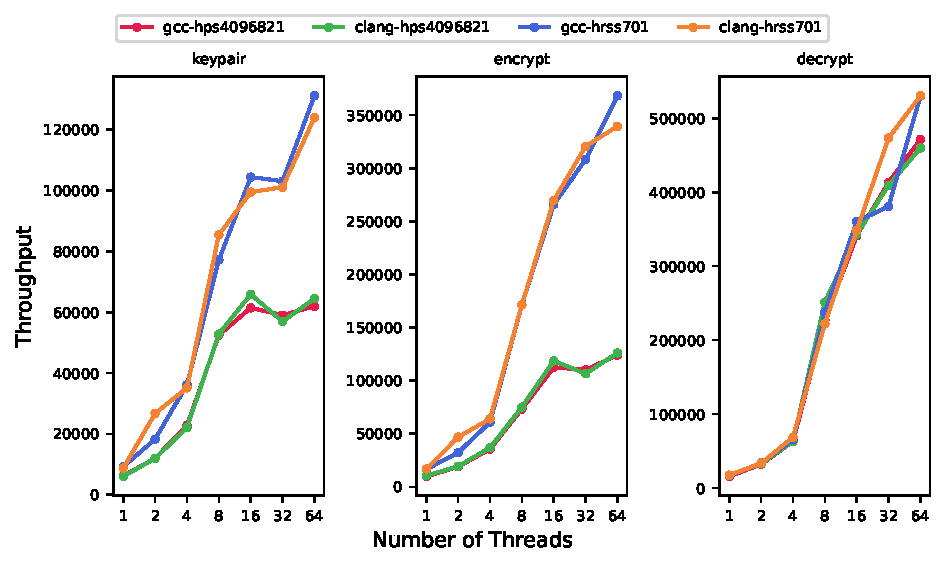
\includegraphics[scale=0.75]{chapters/results/throughput/Modern Workstation_ntru.pdf}
    \caption{Throughput of \gls{ntru} on Modern Workstation}
    \label{figure:results:throughput:ntru:modern-workstation}
\end{figure}

The most inconsistent behavior was found in the Cloud Provider 2 environment, as seen in figure \ref{figure:results:throughput:ntru:cloud-provider-2}. The environment also provided inconsistent throughput for \gls{mceliece} as presented in figure \ref{figure:results:throughput:mceliece:cloud-provider-2}. The dip in throughput previously discussed occuring at roughly 2 times the \gls{smt} number of threads seems to affect the Cloud Provider 2 more than other environments. The same inconsistency was not found in Cloud Provider 1.

\begin{figure}
    \centering
    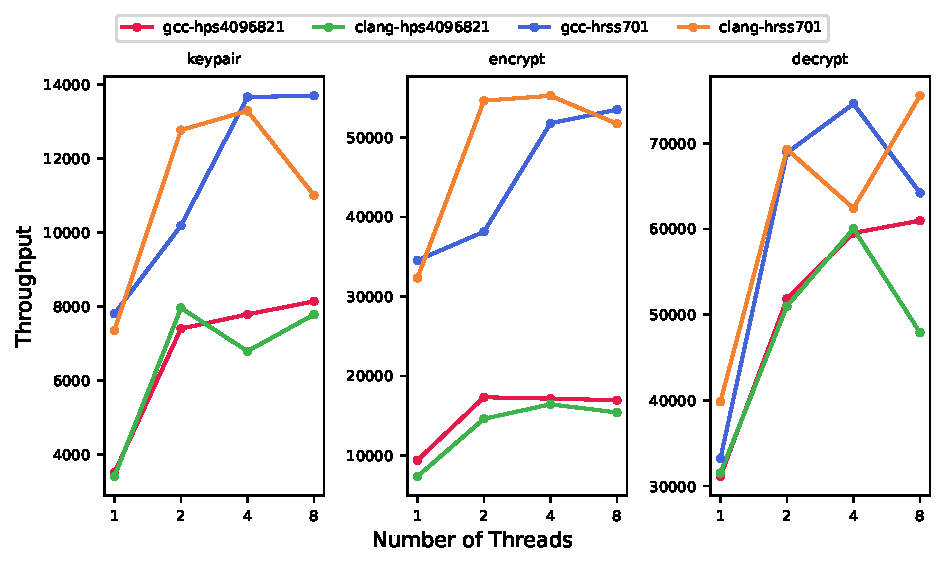
\includegraphics[scale=0.75]{chapters/results/throughput/Cloud Provider 2_ntru.pdf}
    \caption{Throughput of \gls{ntru} on Cloud Provider 2}
    \label{figure:results:throughput:ntru:cloud-provider-2}
\end{figure}

    \begin{table}[H]
        \centering
        \small
        \caption{Parallel Throughput Runs for \gls{dhe} (keypair)}
        \begin{tabularx}{\linewidth}{X c c c c c c c c}
            \toprule
            \thead{Environment} & \thead{Compiler} & \multicolumn{7}{c}{\thead{Threads}}\\
            & & 1 & 2 & 4 & 8 & 16 & 32 & 64 \\
            \midrule
\multirowcell{4}{Cloud\\ Provider\\ 1} & 
\multirow{2}{*}{gcc} & 485 & 940 & 1043 & 1021 & 1052\\
 & & 1.0 & 1.94 & 2.15 & 2.10 & 2.17\\
\cmidrule[0.05em](){3-9} & 
\multirow{2}{*}{clang} & 500 & 962 & 1048 & 1046 & 1053\\
 & & 1.03 & 1.98 & 2.16 & 2.15 & 2.17\\
            \midrule
\multirowcell{4}{Cloud\\ Provider\\ 2} & 
\multirow{2}{*}{gcc} & 261 & 522 & 529 & 547\\
 & & 1.0 & 2.00 & 2.02 & 2.09\\
\cmidrule[0.05em](){3-9} & 
\multirow{2}{*}{clang} & 256 & 537 & 520 & 546\\
 & & 0.98 & 2.06 & 1.99 & 2.09\\
            \midrule
\multirowcell{4}{IBM\\ Community\\ Cloud} & 
\multirow{2}{*}{gcc} & 142 & 284 & 277 & 284\\
 & & 1.0 & 1.99 & 1.95 & 1.99\\
\cmidrule[0.05em](){3-9} & 
\multirow{2}{*}{clang} & 142 & 282 & 276 & 282\\
 & & 1.00 & 1.98 & 1.94 & 1.98\\
            \midrule
\multirowcell{4}{Modern\\ Laptop} & 
\multirow{2}{*}{gcc} & 591 & 1171 & 1978 & 2034 & 1997 & 2027\\
 & & 1.0 & 1.98 & 3.34 & 3.44 & 3.38 & 3.43\\
\cmidrule[0.05em](){3-9} & 
\multirow{2}{*}{clang} & 592 & 1112 & 1854 & 1981 & 1979 & 2026\\
 & & 1.00 & 1.88 & 3.14 & 3.35 & 3.35 & 3.43\\
            \midrule
\multirowcell{4}{Modern\\ Workstation} & 
\multirow{2}{*}{gcc} & 744 & 1481 & 2848 & 5617 & 5544 & 5584 & 5741\\
 & & 1.0 & 1.99 & 3.83 & 7.55 & 7.45 & 7.50 & 7.72\\
\cmidrule[0.05em](){3-9} & 
\multirow{2}{*}{clang} & 743 & 1485 & 2853 & 5621 & 5800 & 5568 & 5737\\
 & & 1.00 & 2.00 & 3.83 & 7.55 & 7.80 & 7.48 & 7.71\\
            \midrule
\multirowcell{4}{Old\\ Low-Range\\ Laptop} & 
\multirow{2}{*}{gcc} & 201 & 402 & 433 & 431 & 433\\
 & & 1.0 & 2.00 & 2.15 & 2.14 & 2.15\\
\cmidrule[0.05em](){3-9} & 
\multirow{2}{*}{clang} & 201 & 402 & 433 & 426 & 433\\
 & & 1.00 & 2.00 & 2.15 & 2.12 & 2.15\\
            \midrule
\multirowcell{4}{Old\\ Mid-Range\\ Laptop} & 
\multirow{2}{*}{gcc} & 252 & 394 & 515 & 516 & 517\\
 & & 1.0 & 1.56 & 2.04 & 2.05 & 2.05\\
\cmidrule[0.05em](){3-9} & 
\multirow{2}{*}{clang} & 253 & 336 & 516 & 517 & 517\\
 & & 1.01 & 1.34 & 2.05 & 2.05 & 2.05 \\
            \bottomrule
        \end{tabularx}
    \end{table}
    
    \begin{table}[H]
        \centering
        \small
        \caption{Parallel Throughput Runs for \gls{ntru} HRSS 701 (keypair)}
        \begin{tabularx}{\linewidth}{X c c c c c c c c}
            \toprule
            \thead{Environment} & \thead{Compiler} & \multicolumn{7}{c}{\thead{Threads}}\\
            & & 1 & 2 & 4 & 8 & 16 & 32 & 64 \\
            \midrule
\multirowcell{4}{Cloud\\ Provider\\ 1} & 
\multirow{2}{*}{gcc} & 10021 & 15345 & 21810 & 22629 & 22963\\
 & & 1.0 & 1.53 & 2.18 & 2.26 & 2.29\\
\cmidrule[0.05em](){3-9} & 
\multirow{2}{*}{clang} & 9918 & 20027 & 22637 & 22997 & 23753\\
 & & 0.99 & 2.00 & 2.26 & 2.29 & 2.37\\
            \midrule
\multirowcell{4}{Cloud\\ Provider\\ 2} & 
\multirow{2}{*}{gcc} & 7805 & 10185 & 13663 & 13696\\
 & & 1.0 & 1.30 & 1.75 & 1.75\\
\cmidrule[0.05em](){3-9} & 
\multirow{2}{*}{clang} & 7352 & 12770 & 13289 & 11005\\
 & & 0.94 & 1.64 & 1.70 & 1.41\\
            \midrule
\multirowcell{4}{IBM\\ Community\\ Cloud} & 
\multirow{2}{*}{gcc} & 137 & 277 & 273 & 275\\
 & & 1.0 & 2.02 & 1.99 & 2.00\\
\cmidrule[0.05em](){3-9} & 
\multirow{2}{*}{clang} & 113 & 226 & 223 & 225\\
 & & 0.82 & 1.64 & 1.62 & 1.64\\
            \midrule
\multirowcell{4}{Modern\\ Laptop} & 
\multirow{2}{*}{gcc} & 7061 & 12686 & 20221 & 33444 & 36381 & 40489\\
 & & 1.0 & 1.80 & 2.86 & 4.74 & 5.15 & 5.73\\
\cmidrule[0.05em](){3-9} & 
\multirow{2}{*}{clang} & 5216 & 12854 & 26546 & 35160 & 38757 & 39734\\
 & & 0.74 & 1.82 & 3.76 & 4.98 & 5.49 & 5.63\\
            \midrule
\multirowcell{4}{Modern\\ Workstation} & 
\multirow{2}{*}{gcc} & 9256 & 18275 & 36193 & 77144 & 104379 & 103050 & 131102\\
 & & 1.0 & 1.97 & 3.91 & 8.33 & 11.28 & 11.13 & 14.16\\
\cmidrule[0.05em](){3-9} & 
\multirow{2}{*}{clang} & 8771 & 26758 & 35118 & 85408 & 99441 & 101059 & 123903\\
 & & 0.95 & 2.89 & 3.79 & 9.23 & 10.74 & 10.92 & 13.39\\
            \midrule
\multirowcell{4}{Old\\ Low-Range\\ Laptop} & 
\multirow{2}{*}{gcc} & 124 & 251 & 267 & 267 & 267\\
 & & 1.0 & 2.01 & 2.15 & 2.14 & 2.15\\
\cmidrule[0.05em](){3-9} & 
\multirow{2}{*}{clang} & 63 & 127 & 135 & 135 & 135\\
 & & 0.51 & 1.02 & 1.08 & 1.09 & 1.09\\
            \midrule
\multirowcell{4}{Old\\ Mid-Range\\ Laptop} & 
\multirow{2}{*}{gcc} & 159 & 299 & 319 & 320 & 320\\
 & & 1.0 & 1.88 & 2.01 & 2.01 & 2.01\\
\cmidrule[0.05em](){3-9} & 
\multirow{2}{*}{clang} & 81 & 154 & 163 & 165 & 165\\
 & & 0.51 & 0.97 & 1.03 & 1.04 & 1.04 \\
            \bottomrule
        \end{tabularx}
    \end{table}
    


%          Modern Workstation &                  gcc &                  ref &  0.91ms &                  0.0\\
%          Modern Workstation &                  gcc &        ref-optimized &  0.23ms &                  2.9\\
%          Modern Workstation &                clang &        ref-optimized &  0.21ms &                  3.4\\
%          Modern Workstation &                  gcc &                 avx2 &  0.03ms &                 30.8\\
%          Modern Workstation &                  gcc &       avx2-optimized &  0.02ms &                 49.7\\
%          Modern Workstation &                clang &       avx2-optimized &  0.02ms & 


\section{Lek Stuga}
\begin{table}[H]
        \centering
        \small
        \caption{Parallel Throughput Runs for ntru hrss701}
        \begin{tabularx}{\linewidth}{X c c c c c c c}
            \toprule
            \thead{Environment} & \thead{Compiler} & \multicolumn{3}{c}{\thead{Average Duration}} & \multicolumn{3}{c}{\thead{Speedup}}\\
            & & keypair & encrypt & decrypt & keypair & encrypt & decrypt \\
            \midrule
\multirowcell{4}{Cloud\\ Provider\\ 1} & 
\multirow{2}{*}{gcc} & 10021 & 15345 & 21810 & 22629 & 22963\\
 & & 1.0 & 1.53 & 2.18 & 2.26 & 2.29\\
\cmidrule[0.05em](){3-8} & 
\multirow{2}{*}{clang} & 9918 & 20027 & 22637 & 22997 & 23753\\
 & & 0.99 & 2.00 & 2.26 & 2.29 & 2.37\\
 
            \bottomrule
        \end{tabularx}
    \end{table}